\documentclass[12pt,a4paper]{article}
\usepackage[utf8]{inputenc}
\usepackage[german]{babel}
\usepackage[T1]{fontenc}
\usepackage{amsmath}
\usepackage{amsfonts}
\usepackage{amssymb}
\usepackage{graphicx}
\usepackage{siunitx}
\usepackage{float}
\usepackage[left=2cm,right=2cm,top=2cm,bottom=2cm]{geometry}
\author{Gerald}

\begin{document}
\sisetup{separate-uncertainty = true}
	\setlength{\parindent}{0pt} 
	\begin{center}
		{\LARGE Versuchsprotokoll}\\
		\begin{large}
			zum Fortgeschrittenenpraktikum im Bachelorstudiengang Physik\\[0.4cm]
			an der RWTH Aachen\\
			II. Physikalisches Institut A\\[5.5cm]
			\Large\textbf{\textsl{Nuclear Magnetic Resonance (NMR)}}\\[5.5cm]
			\normalsize\textit{vorgelegt\\von}\\[0.4cm]
			\large{Moritz Berger\\Gerald Kolter}\\[2cm]
			\large \textbf{Wintersemester 2017/18}
		\end{large}
	\end{center}
	\newpage
	
	\tableofcontents
	\newpage

\section{Ziel des Versuchs}
Das Ziel des Versuches besteht darin, die Relaxationszeiten von Wasserstoffkernen, also von Protonen, zu bestimmen. Diese geben an, wie schnell sich die Spins nach Auslenkung wieder in Richtung eines konstanten Magnetfeldes ausrichten.\\
Wenn sich Spins in einem konstanten Magnetfeld (im Folgenden mit $B_0$ bezeichnet) befinden, richten sie sich entlang dessen aus. Durch Anlegen eines Wechselfeldes (im Folgenden mit $B_1$ bezeichnet) senkrecht dazu, wird das effektive Magnetfeld zur Vektoraddition zwischen dem konstanten Magnetfeld und dem Wechselfeld. Die Spins präzedieren dann um das effektive Magnetfeld. Wird das Wechselfeld nur kurz angelegt, drehen die Spins keine ganze Rotation um das effektive Magnetfeld. Dadurch kann die Ausrichtung der Spins manipuliert werden. Im Folgenden sind sogenannte $\pi /2$-Pulse und $\pi$-Pulse relevant. Diese bezeichnen Pulse des Wechselfeldes, die die Spins um einen Winkel von $\pi /2$ bzw. $\pi$ drehen.\\
Bei der Wahl des Koordinatensystems wird die Z-Achse in Richtung des konstanten Magnetfeldes $B_0$ gelegt. Für die Betrachtung der Spinausrichtung wird in ein sich mit dem Spin um die z-Achse rotierendes Koordinatensystem gewechselt, sodass der Spin ein konstanter Vektor ist. Wenn die Frequenz der Pulse der Frequenz, mit der die Spins rotieren, der sogenannten Larmorfrequenz $\omega _L = \gamma \cdot B_0$ mit dem gyromagnetischen Verhältnis $\gamma$ entspricht, bewirkt ein $\pi /2$-Puls eine Drehung des Spins in die x-y-Ebene. Ein $\pi$-Puls spiegelt den Spin an der x-y-Ebene.


\section{Aufbau}
In ein konstantes Magnetfeld eines Permanentmagneten wird eine Spule so installiert, dass die Magnetfeldrichtung eines durch Induktion in dieser Spule erzeugten Magnetfeldes senkrecht auf dem Feld des Permanentmagneten steht. In diese Spule wird die Probe eingebracht. \\
Die Spule dient gleichzeitig als Sender für ein Wechselfeld und als Messinstrument für die Magnetisierung in der Richtung der Spule, da diese in der Spule einen Strom induziert.\\
Mit einem Frequenzgenerator wird ein elektrisches Wechselfeld erzeugt, das wiederum ein Magnetfeld in der Spule induziert. Da zeitlich kurze Magnetfelder benötigt werden, wird der Frequenzgenerator an einen Pulsgenerator angeschlossen. Der dadurch generierte Wechselfeldpuls wird auf die Spule gegeben. Der Pulsgenerator dient gleichzeitig als Triggersignal für das Oszilloskop.\\
Das elektrische Signal, das in der Spule durch die Magnetisierung induziert wird, wird in einem sogenannten Mixer mit dem Signal des Frequenzgenerators multipliziert. Dieses Signal wird auf dem Oszilloskop zusammen mit dem direkt aus der Spule entnommenen Signal angezeigt.\\
Der Verstärker bietet die Möglichkeit, die Verstärkung für einen kurzen Zeitraum auf Null zu stellen, das sogenannte blanking. Damit können die Pulse aus dem Oszilloskopbild rausgehalten werden.



\section{Durchführung}

\subsection{Vorversuche}
Vor der eigentlichen Messung müssen die Versuchsparameter richtig gewählt werden. Dazu wird anstelle der Probe eine kleine Spule, die anstelle der Empfängerspule an das Oszilloskop angeschlossen wird, in den Probenraum eingebracht. Dann werden die Frequenz ($\omega _p$) und die Höhe der Leiterschleife variiert, bis der induzierte Strom in der Leiterschleife maximal ist. Bei bekannten Größen der Leiterschleife (Querschnittsfläche $A$ und Anzahl Windungen $N$) kann daraus die Stärke des Wechselfeldes $B_1$ bestimmt werden:
\begin{equation*}
B_1 = \dfrac{U_0}{2 \omega _p N A}
\end{equation*}
Wenn die Frequenz $\omega _p \approx \omega _L$ gefunden ist, die Länge des $\pi /2$-Pulses bestimmt werden:
\begin{equation}
\label{T_pi/2}
T_{\pi /2} = \dfrac{\pi}{2} \cdot \dfrac{1}{\omega _p} = \dfrac{\pi}{2 \omega _p} = \dfrac{\pi}{2 \gamma B_1} = \dfrac{\pi N A \omega _p}{\gamma U_0}
\end{equation}
Wobei das gyromagnetische Verhältnis gegeben ist zu:
\begin{equation*}
\gamma _{Proton} = 2,675 \cdot 10^{8} \dfrac{1}{T s} 
\end{equation*}
Der $\pi$-Puls ist entsprechend doppelt so lang wie der $\pi /2$-Puls.\\
Mit diesen Voreinstellungen können nun die korrekten Parameter gewählt werden. Dazu wird die Probe in den Probenraum eingebracht. Der Einfachheit halber auf der Höhe, auf der vorher die Spule war. In dem direkten Signal aus dem Probenraum sollte nun gemäß Additionstheorem eine Schwebung
\begin{equation*}
2 \cdot \cos (\omega _L t) \cdot \cos (\omega _p t) = \cos ((\omega _L + \omega _p) t) \cdot \cos ((\omega _L - \omega _p) t)
\end{equation*}
zu sehen sein, wobei nur der Anteil mit der geringeren Frequenz zu sehen ist ($\propto \cos ((\omega _L - \omega _p) t)$). Wenn in den Daten keine Schwingung mehr zu sehen ist, ist damit offensichtlich der Punkt $\omega _p = \omega _L$ gefunden. Um diesen Punkt zu finden, müssen die Höhe der Probe, die Frequenz und mit der Frequenz gemäß Gl. \ref{T_pi/2} auch die Pulsdauer variiert werden.\\
Die einzustellenden Parameter sind abhängig von der Frequenz, die wiederum abhängig von der Stärke des konstanten Magnetfeldes ist. Da der Permanentmagnet temperaturabhängig ist, muss die Feineinstellung der Parameter zwischen den Messreihen wiederholt werden.


\subsection{Messung von T1}

\begin{figure}
\centering
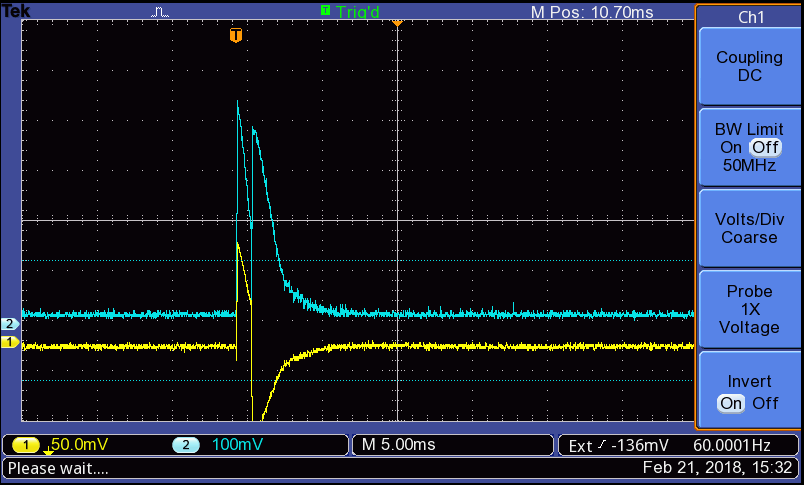
\includegraphics[scale=0.8]{Bilder/F0003TEK.PNG}
\caption{Ergebnis einer einzelnen Messung zur Bestimmung von T1. Die blaue Kurve zeigt das zu untersuchende Signal.}
\label{fig:MessungT1_Beispiel}
\end{figure}

Für die Messung von T1 werden die Spins mit einem $\pi$-Puls umgedreht. Nach einer Wartezeit $\tau$, werden die restlichen, noch in der umgedrehten Position befindlichen Spins mit einem $\pi /2$-Puls in die x-y-Ebene gedreht, um dort vermessen zu werden. Das Ergebnis einer solchen Messung ist beispielhaft in Abbildung \ref{fig:MessungT1_Beispiel} gezeigt. Der erste Peak ist der Rest des $\pi$-Pulses. Der zweite Peak ist der Free Induction Decay (FID) nach dem $\pi /2$-Puls. \\
Für die Bestimmung von T1 wird die Wartezeit zwischen den beiden Pulse durchgefahren und die relative Höhe des FID zur Höhe des $\pi$-Pulses bestimmt. Die Erwartung ist ein exponentieller Abfall:
\begin{equation}
\label{eq:T1_Exponentialfunktion}
U_{rel} (t) := \dfrac{U_{FID} (t)}{U_0} = 1 - 2 e^{-\frac{t}{T_1}}
\end{equation}




\subsection{Messung von T2}


\section{Ergebnisse}

\subsection{T1}
Es wird immer nur der Betrag des FID-Signals angezeigt, daher muss der Teil der Messwerte, die vor dem Nulldurchgang liegen noch mit dem Faktor (-1) multipliziert werden. In Tabelle \ref{tab:T1_Daten} ist dies bereits geschehen. Genauso ist der Offset bereits korrigiert.

\begin{table}
\centering
\begin{tabular}{|c|c|c|}
\hline 
Pulshöhe [mV] & FID-Höhe [mV] & $\tau$ [s] \\ 
\hline 
448 & -396 & 0.918 \\ 
\hline 
452 & -380 & 1.800 \\ 
\hline 
452 & -356 & 2.700 \\ 
\hline 
472 & -328 & 3.618 \\ 
\hline 
472 & -296 & 4.554 \\ 
\hline 
452 & -268 & 5.436 \\ 
\hline 
460 & -236 & 6.300 \\ 
\hline 
448 & -204 & 7.290 \\ 
\hline 
460 & -176 & 8.154 \\ 
\hline 
456 & -136 & 9.036 \\ 
\hline 
456 & -124 & 9.954 \\ 
\hline 
452 & -92 & 10.854 \\ 
\hline 
444 & -72 & 11.862 \\ 
\hline 
456 & -52 & 12.978 \\ 
\hline 
448 & -40 & 13.428 \\ 
\hline 
440 & -36 & 14.040 \\ 
\hline 
444 & -32 & 14.148 \\ 
\hline 
452 & -28 & 14.490 \\ 
\hline 
448 & 28 & 14.850 \\ 
\hline 
448 & 44 & 15.300 \\ 
\hline 
440 & 40 & 15.516 \\ 
\hline 
440 & 52 & 15.858 \\ 
\hline 
448 & 60 & 16.326 \\ 
\hline 
440 & 56 & 17.118 \\ 
\hline 
448 & 80 & 18.000 \\ 
\hline 
444 & 108 & 18.864 \\ 
\hline 
444 & 128 & 19.818 \\ 
\hline 
452 & 136 & 20.718 \\ 
\hline 
444 & 160 & 21.636 \\ 
\hline 
452 & 176 & 22.500 \\ 
\hline 
440 & 196 & 23.400 \\ 
\hline 
432 & 200 & 24.336 \\ 
\hline 
444 & 212 & 25.218 \\ 
\hline 
436 & 228 & 26.100 \\ 
\hline 
444 & 248 & 27.090 \\ 
\hline 
416 & 252 & 27.990 \\ 
\hline 
420 & 260 & 28.800 \\ 
\hline 
424 & 272 & 29.700 \\ 
\hline 
432 & 296 & 30.600 \\ 
\hline 
404 & 300 & 30.690 \\ 
\hline 
416 & 292 & 31.500 \\ 
\hline 
412 & 304 & • \\ 
\hline 
412 & 364 & • \\ 
\hline 
\end{tabular} 
\caption{Messwerte der Höhen des $\pi /2$-Pulses und des FID s beim Durchfahren von $\tau$ zur Bestimmung von T1.}
\label{tab:T1_Daten}
\end{table}


\subsubsection{Rauschmessung}
Wie in Abbildung \ref{fig:MessungT1_Beispiel} gut zu erkennen ist, ist ein deutliches Hintergrundrauschen vorhanden. Aus diesem lässt sich ein Offset bestimmen, der zur Korrektur der Höhen wichtig ist, und ein statistischer Fehler auf die Spannungsmessung. Die Ergebnisse sind:
\begin{equation*}
\sigma _U = ????
\end{equation*}
\begin{equation*}
U_{offset} = ????
\end{equation*}


\subsubsection{Zero-crossing-point-Methode}
Anhand von Gl. \ref{eq:T1_Exponentialfunktion} lässt sich leicht ersehen, dass aus dem Punkt an dem die Daten die Nulllinie durchqueren $T_1$ abgeschätzt werden kann als:
\begin{equation*}
T_1 = \dfrac{1}{ln(2)} \cdot T_{U_{rel} = 0}
\end{equation*}
Für die Fehlerabschätzung muss ein Fehler auf den Nulldurchgang ermittelt werden. Anhand der Daten ist gut ersichtlich, dass der Nulldurchgang irgendwo zwischen den Werten $T_{U_{rel} < 0} = 13.428ms$ und $T_{U_{rel} > 0} = 15.516ms$ liegt. Damit ergibt sich der Messwert für T1 zu:
\begin{equation*}
T_1 = \dfrac{1}{ln(2)} \cdot \dfrac{T_{U_{rel} > 0} - T_{U_{rel} < 0}}{2} = 20.879 ms
\end{equation*}
\begin{equation*}
\sigma _{T_1} = \dfrac{1}{ln(2)} \cdot \dfrac{T_{U_{rel} > 0} - T_{U_{rel} < 0}}{\sqrt{12}} = 0.870 ms
\end{equation*}

\subsubsection{Linearer Fit an halblogarithmischer Auftragung}
Formt man Gl. \ref{eq:T1_Exponentialfunktion} zu einer linearen Funktion um, ergibt sich:
\begin{equation}
ln(1 - U_{rel} (t)) = -\dfrac{t}{T_1} + ln(2)
\label{eq:T1_linFunktion}
\end{equation}
Daher kann durch geeignete Auftragung eine lineare Funktion an die Daten gefittet werden. Mittels Fehlerfortpflanzung ergibt sich für die Fehler auf die Y-Koordinate:
\begin{equation}
\sigma _y = \sigma _{U_{rel}} \cdot \dfrac{1}{1 - U_{rel}}
\end{equation}
Dabei bestimmt sich der Fehler auf $U_{rel}$ zu:
\begin{equation*}
\sigma _{U_{rel}} = \sigma _U \cdot \sqrt{\left(\dfrac{1}{U_Puls - offset}\right)^2 + \left(\dfrac{U_{FID} - offset}{(U_{Puls} - offset)^2}\right)^2}
\end{equation*}


\subsubsection{Exponentialfit}



\subsection{T2}


\end{document}